
\begin{sidewaysfigure}
\centering
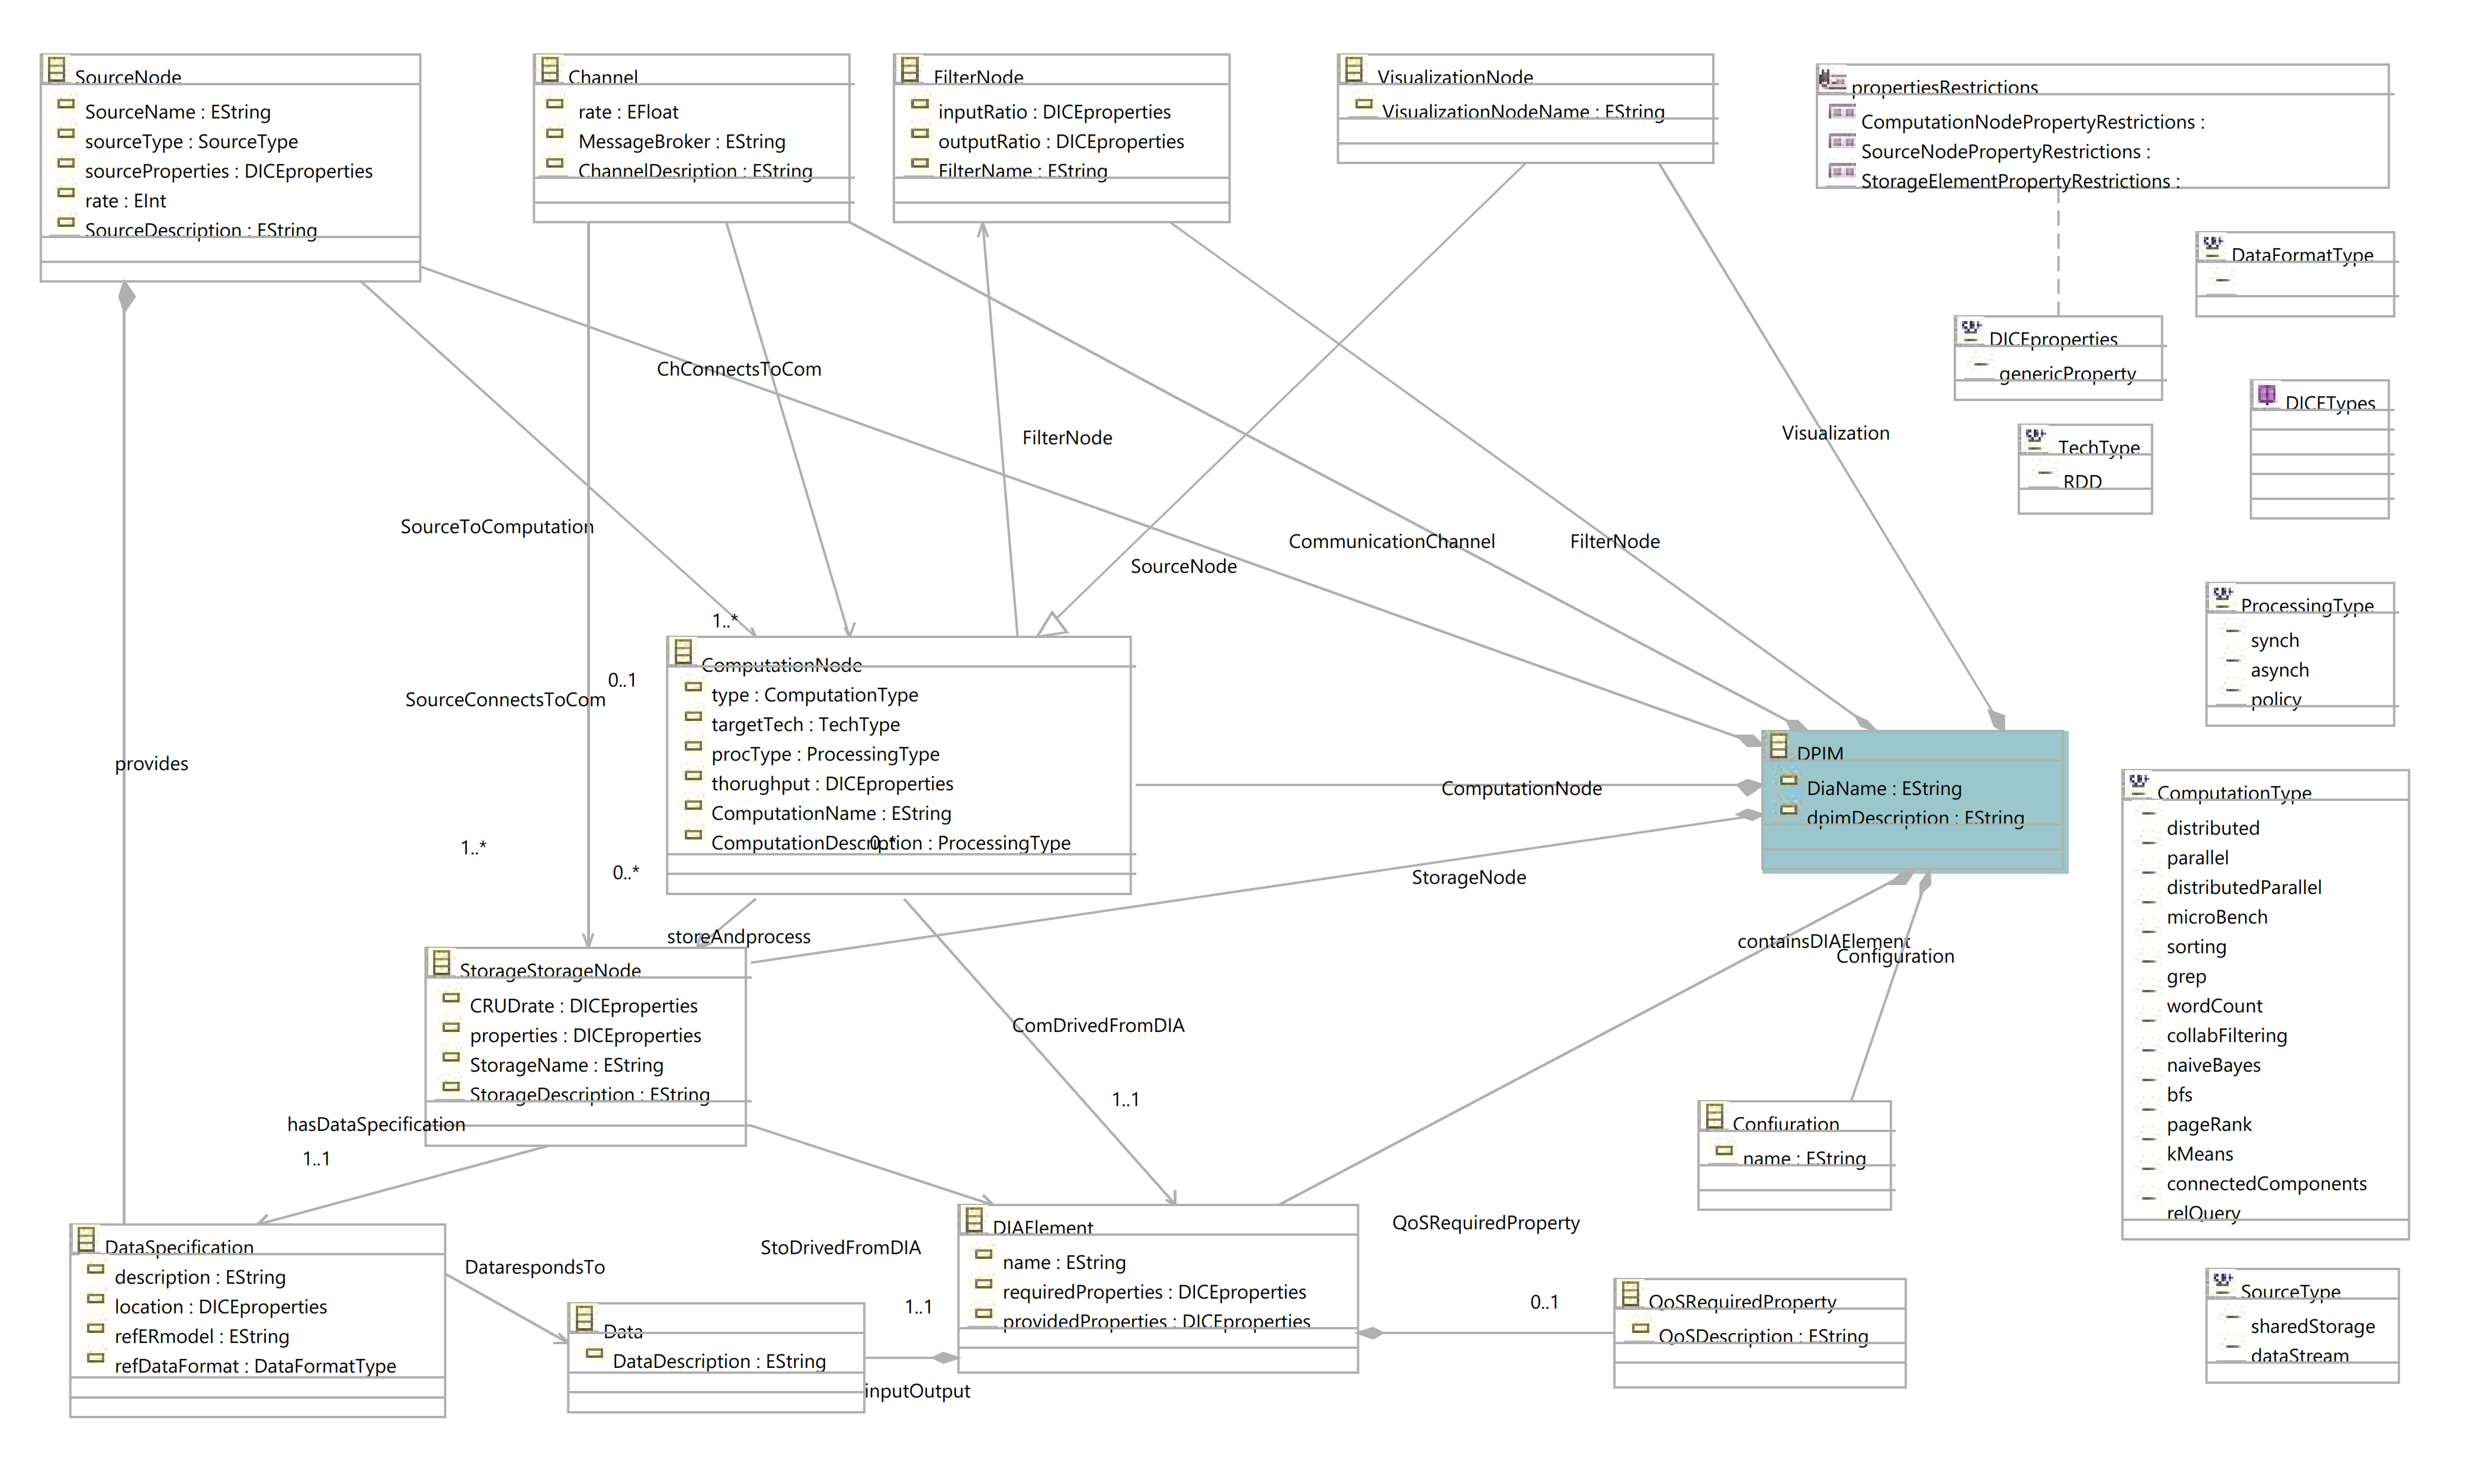
\includegraphics[width=\textwidth]{Images/11.png}
\caption{\label{fig:metamodel}DICE DPIM metamodel.}
\end{sidewaysfigure}

\begin{figure}
\centering
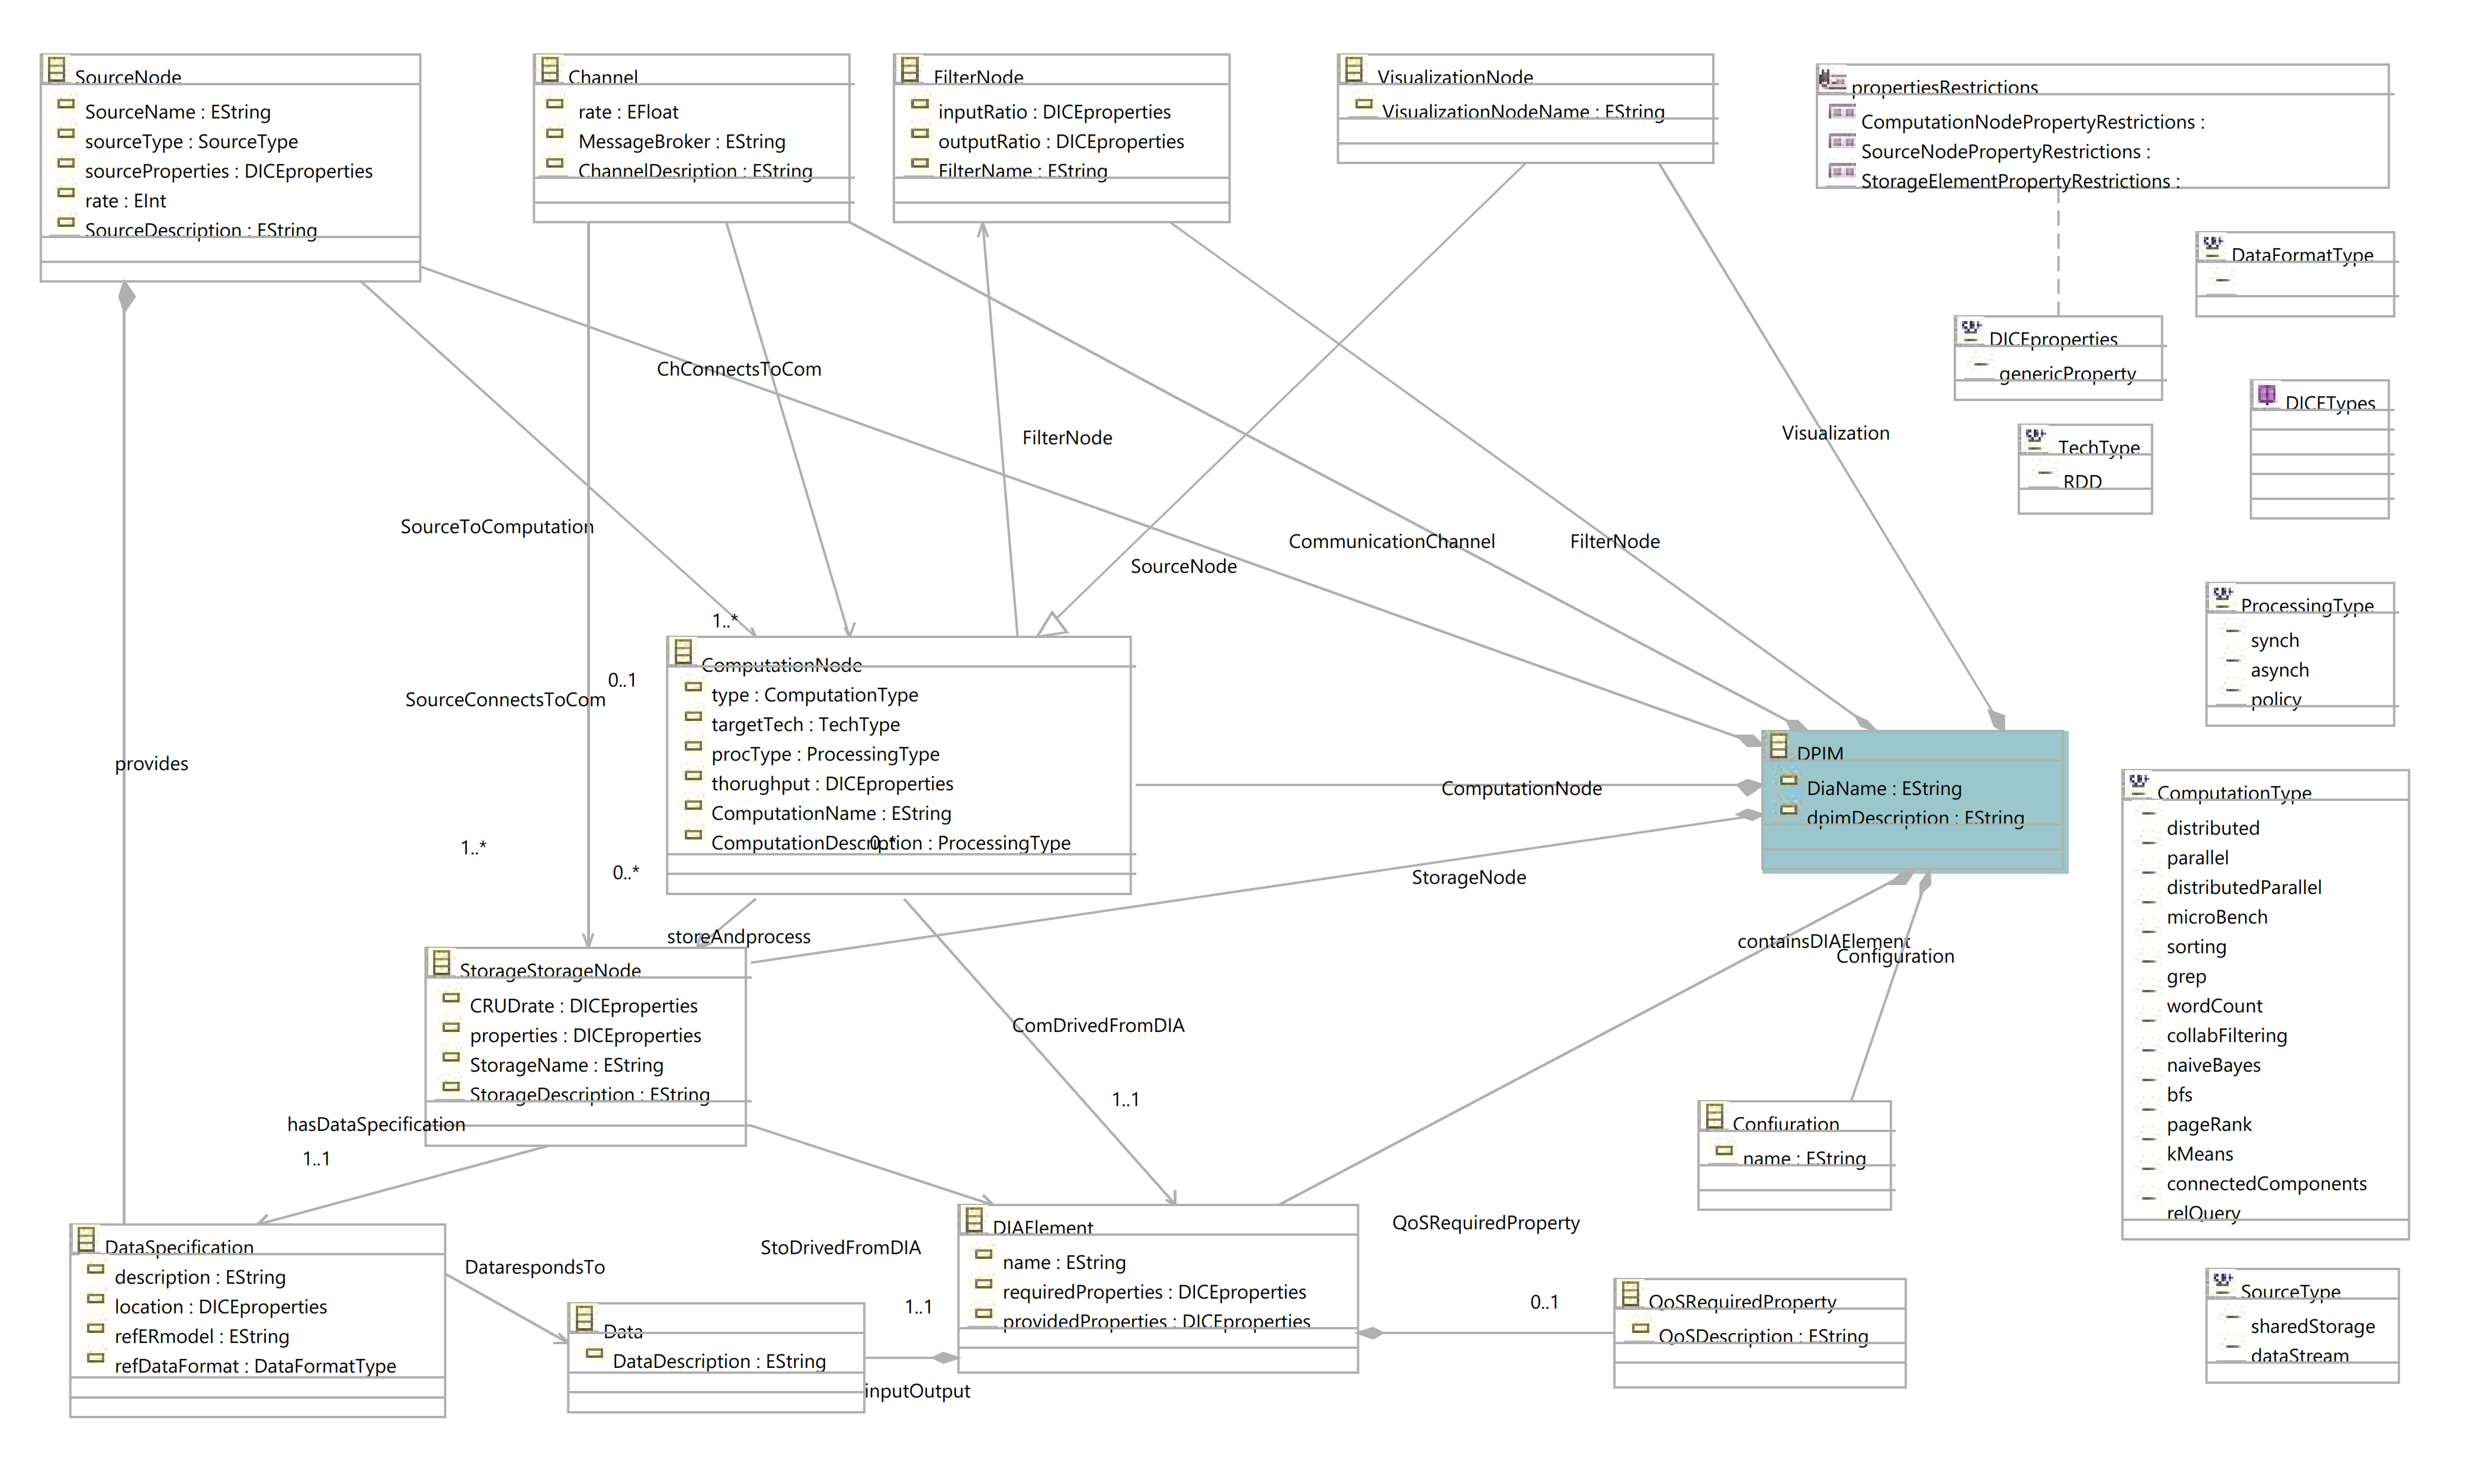
\includegraphics[width=\textwidth]{Images/11.png}
\caption{\label{fig:metamodel2}DICE DPIM metamodel in portrait form.}
\end{figure}


\subsection{Product perspective}

\subsubsection{User interfaces}

\begin{itemize}
	\item A new user should be able to make an account, without training, in less than 10 minutes
	\item The number of steps requested to user in "appointment creation" should be less than 5
	\item User should be allowed to access system functions from mobile devices such as smart-phone and tablets
	\item User should be allowed to access system functionalities from PC
	\item UI for mobile devices should adapt to different screen sizes (from 5 to 11 inch)
	\item There shouldn't be need of training for new user to learn all application functionalities offered by UI
\end{itemize}
\subsubsection{System interfaces}

System have to communicate with external services, from public transportation means to map services. In order to guarantee future support to new services, also outside Milan area, it ought to be useful a modular, flexible but also extendible approach on the building of external interface. In the following part of the paragraph it will be shown a list of logic operation that should be accomplished by external services APIs in order to be interfaced and employed by the system.

\begin{itemize}
	\item Train services and trams
	\subitem Looking for station list
	\subsubitem System request: station list
	\subsubitem Service response: list of station with locations
	
	\subitem Looking for train/tram
	\subsubitem System request: departure and arrival stations, departure time
	\subsubitem list of possible rides, cost of travel, times of leaving and arrival (at least 1 list's element)
	
	\item Taxi
	\subitem Looking for taxi
	\subsubitem System request: departure position and time
	\subsubitem Service response: disponibility and (hourly or journey cost)
	
	\item Bike sharing
	\subitem Looking for service parking spot
	\subsubitem System request: spaces
	\subsubitem Service response: list of spaces with available bicycles
	\subitem Looking for fees
	\subsubitem System request: fees
	\subsubitem Service response: hourly fee
	
	\item Map services
	\subitem System should be able to retrieve the nearest address given GPS coordinates and vice-versa by these services.
	\subitem Map services should be able to generate a route between two given address on system request.
	\subitem System should be allowed to download a portion of map.
	
	\item Weather forecast service
	\subitem Request forecast
	\subsubitem System request: forecast for a specific location and time
	\subsubitem Service response: weather conditions and temperature for requested locality and time
	
	
\end{itemize}

\subsubsection{Software interfaces}

In order to ship a complete functional software, at least for the city of Milan, a list of required supported external APIs is provided in this paragraph.

\begin{itemize}
	\item Trenitalia
	\subitem Name: “Informazioni-Treni-Italiani”
	\subitem Description: unofficial API for Trenitalia, further details on source
	\subitem Version: testing
	\subitem Source: \url{https://github.com/Razorphyn/Informazioni-Treni-Italiani}
	
	\item ATM
	\subitem Name: “localizzazione delle fermate delle linee urbane di superficie”
	\subitem Description: list of metro stops and hours in data-sheet version, regularly updated
	\subitem Version: 29/12/2015
	\subitem Source: \url{http://dati.comune.milano.it/}
	
	\item Bike Sharing
	\subitem Name: “Mobilità: localizzazione delle rastrelliere per il bike sharing”
	\subitem Description: list of bikesharing areas in datasheet version, regularly updated
	\subitem Version: 05/12/2016
	\subitem Source: \url{http://dati.comune.milano.it/}
	
	\item Taxi
	\subitem Name: “appTaxi | Developers”
	\subitem Description: restricted API to book or calculate prices for a ride
	\subitem Version: rolling
	\subitem Source: \url{www.apptaxi.it/developers/}
	
	\item Weather
	\subitem Name: “Open Weather Map API”
	\subitem Description: open API to get weather conditions for a location
	\subitem Version: rolling
	\subitem Source: \url{https://openweathermap.org/api}
	
\end{itemize}
\subsection{Product functions}

It has been selected a set of functionalities, on one hand in order to provide to user a service that focus on easy of use, automation and simplification of user processes and interactions with the system, on the other hand allowing him to freely compose complex schemes of constraints in the choice of travel routes.

\subsubsection{Preference profile creation}
A logged user should be able to create some types of constraints (flexible launch, disabilitation of transport means, set pauses from transport and maximum travelling distance by types of transport mean). He should also be allowed to create many different preferences profiles, that are logical containers for sets of user preferences. These profiles can be applied to single appointments personalizing the research of a routes. Preferences with unspecified profiles belongs to “default” profile and they will ever be considered as constraint for route generation.

\subsubsection{Appointment insertion}

A user can register an appointment providing a description, a date, a time of begin and end. Beside, a registered user can optionally add a list of preferences profiles. The appointment shouldn’t conflict with others of the same user, so if it happens, it will be rejected. Accepted appointment have to be processed, and route options prompted to user.

\subsubsection{Appointment modification}

A user can modify any detail of a previous inserted appointment. If the user is logged into the system, all modifications have to be synchronized with user account.
Finally, system should provides new routes for reaching the modified appointment, deleting previous saved routed linked with the old one.

\subsubsection{Change travel route}

A user can choose to change a saved route. In this case, system will delete user current selected saved route and it will provides new routes to user.

\subsubsection{Route choice}

When requested, the system have to generate routes to reach appointment according to registered user preferences profiles and the previous appointment. System will provide a route that will minimize distance, another one minimizing duration and others minimizing carbon footprint or number of changes.

\subsubsection{User Registration}

User can choose to register an account into the system through MA indicating a valid email address, a secure password, name, surname and fiscal code. 

\subsubsection{User login}

A registered user can log in using phone number and sms verification process or by email and password.



\subsection{User characteristics}

It’s possible to divide application users into two groups:

\begin{itemize}
	\item Unregistered
	\subitem He can access some app features, including appointment registration and route choices
	\item Registered
	\subitem He can access all the feature set that system can provide, so all the functionality provided to unregistered user, plus the possibility to set profiles of preferences, synchronization and backup of user data and preferences. This user can also receive weather forecast update.
\end{itemize}

The user of this system is not required to have IT skills.

\subsection{Assumptions}

{GET FROM EXTERNAL DOC}
